\chapter{Introducción}
\label{chap:intro}
En este capítulo se introducen los conceptos básicos en robótica, de como esta nos ayuda en nuestro día a día, y cual es su estado actual. Y como puede ser un gran recurso en la educación, y de las principales características de la robótica educativa.

\section{Robótica}
\label{sec:robotica}
La robótica es una rama de las ingenierías y de las ciencias de la computación que se encarga del diseño, construcción, operación, estructura, manufactura y aplicación de los robots.
El término \textit{robot} se popularizó con el éxito de la obra R.U.R. (\textit{Robots Universales Rossum}), escrita por Karel Čapek en 1920. En la traducción al inglés de dicha obra la palabra checa \textit{robota}, que significa trabajos forzados o trabajador, fue traducida al inglés como robot.
Un robot es una entidad virtual o mecánica artificial. Están diseñados con un propósito propio.La independencia creada en sus movimientos hace que sus acciones sean la razón de un estudio razonable y profundo en el área de la ciencia y tecnología. La palabra robot puede referirse tanto a mecanismos físicos como a sistemas virtuales de software, aunque suele aludirse a los segundos con el término de bots.

    \begin{figure}[H]
    \centering
    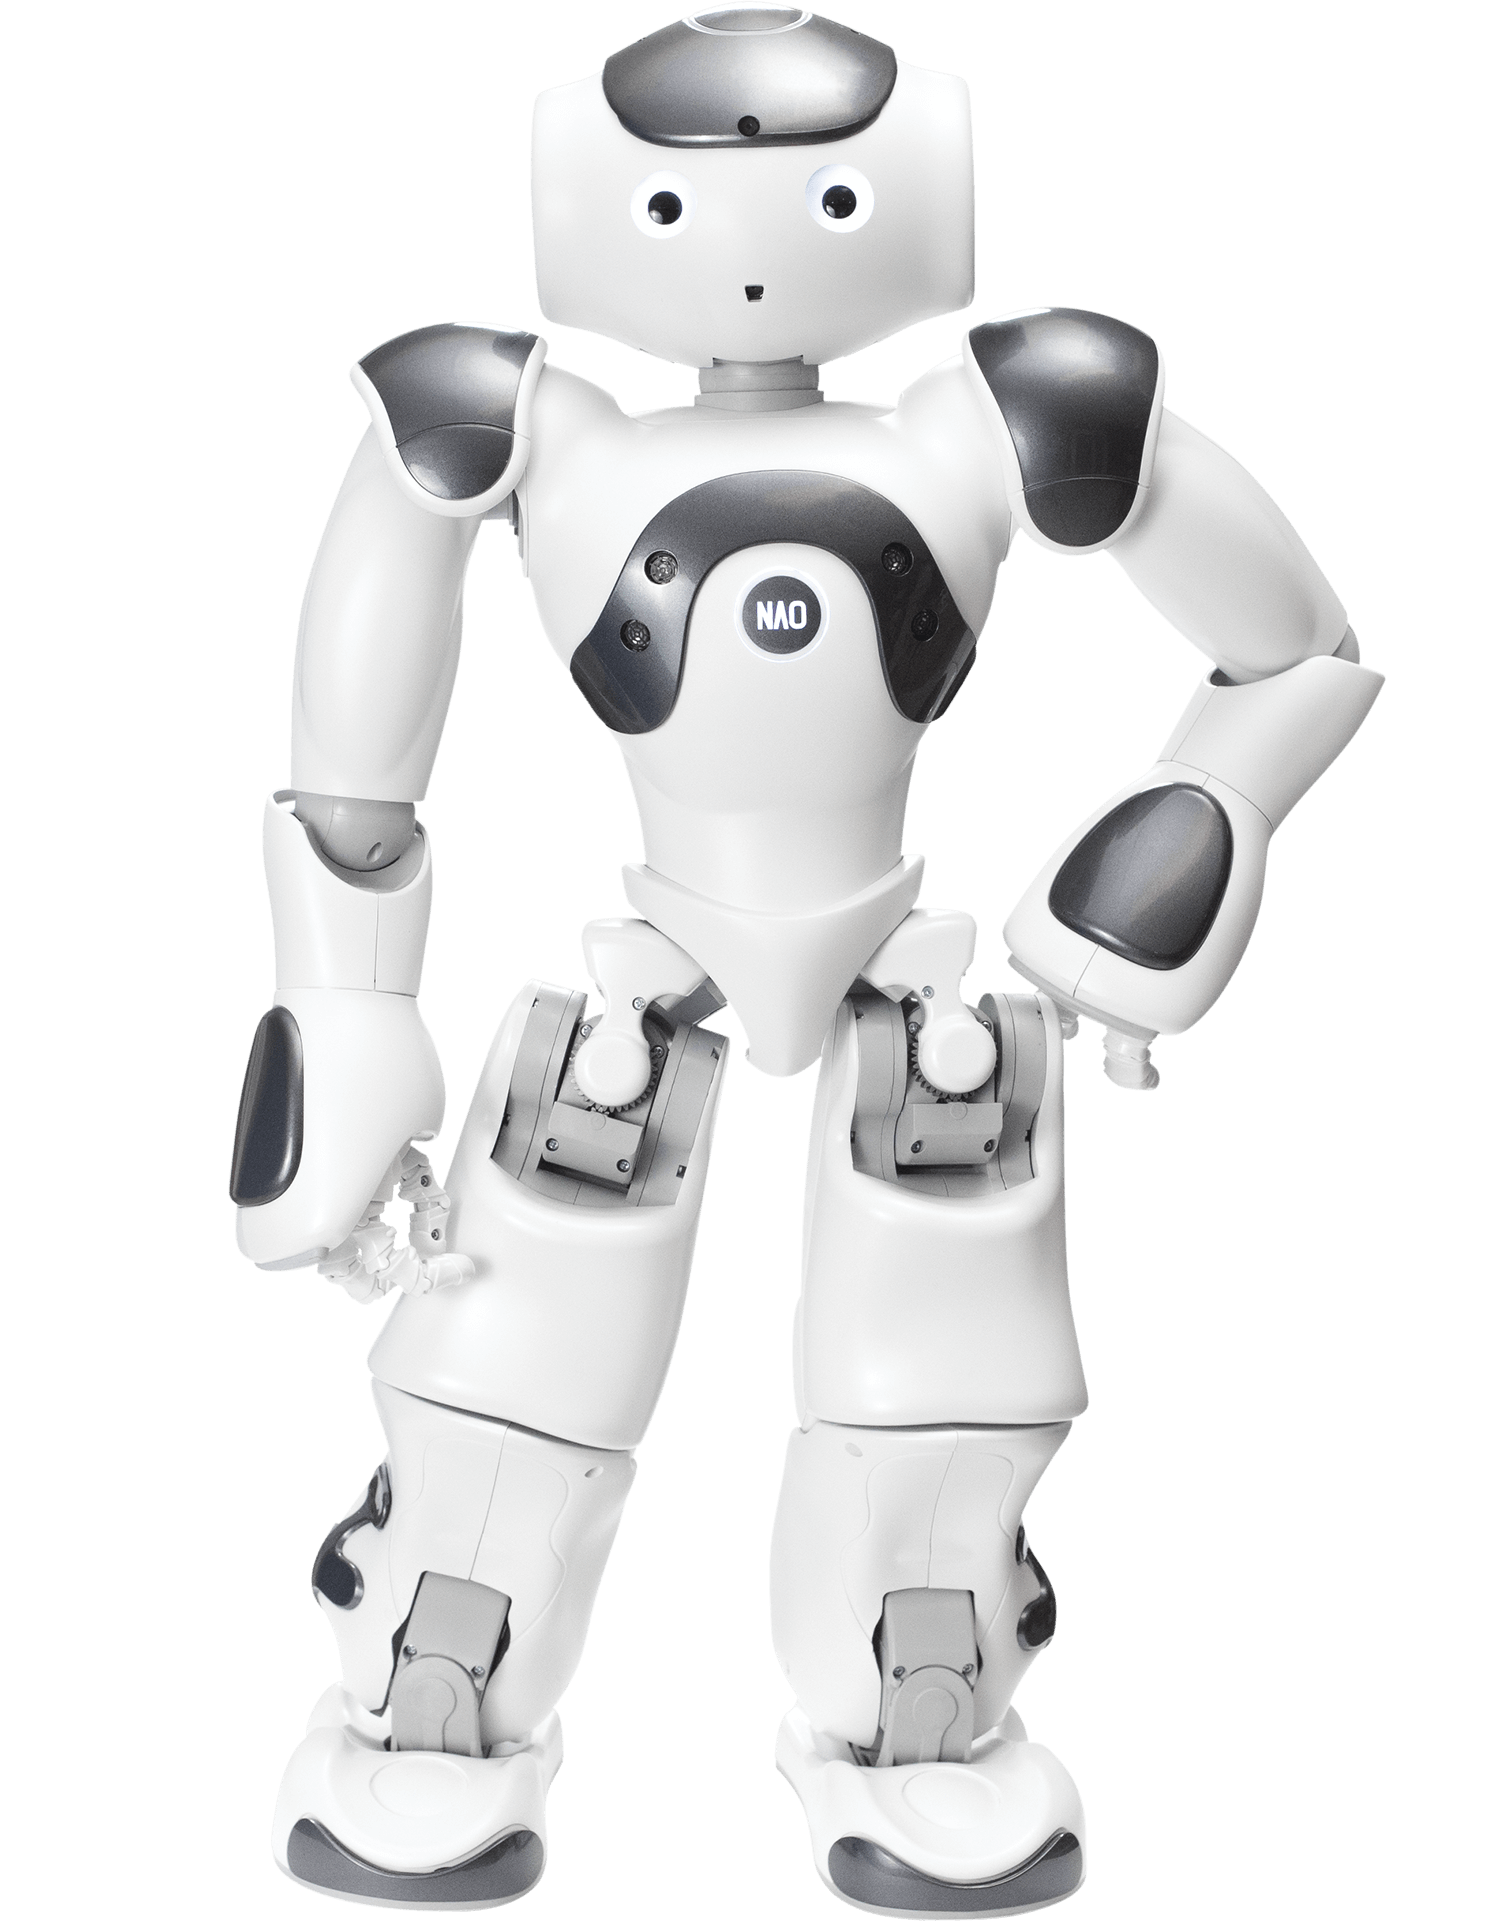
\includegraphics[width=0.8\textwidth]{img/robot.png}
    \caption{Imagen clásica de un robot} \label{fig:robot}
    \end{figure}

No hay un consenso sobre qué máquinas pueden ser consideradas robots,
dentro de este proyecto tomaremos como definición que un robot es un sistema autónomo programable capaz de realizar tareas complejas. Además, todos los robots se componen de tres partes esenciales  se componen de sensores, controladores y actuadores.
\begin{itemize}
    \item \textbf{Sensores}: Son los sentidos del robot, con ellos ve, escucha y sabe lo que hay en el entorno. Recogen la información necesaria para que el robot realice la tarea En este grupo se encuentran láseres, cámaras, ultrasonidos u odómetros..
    \item \textbf{Controladores}: El equivalente al cerebro humano, utiliza los datos recogidos por los sensores para elaborar una respuesta para que la lleve acabo los actuadores.
    \item \textbf{Actuadores}: Equivalen a los músculos humanos, son los que se encargan de interactuar con el entorno para llevar a cabo su tarea. Son brazos mecánicos, motores, etcétera...
\end{itemize}

\subsection{Aplicaciones robóticas}

Ahora que tenemos las bases de lo que es un robot asentadas podemos hablar de cuales son los principales propósitos de los robots hoy en día,aunque la mayor parte de ellos son utilizados por empresas en labores industriales. Aunque hay otros que podemos encontrar en nuestra vida cotidiana, en casas, hospitales, almacenes de tiendas... Esto es debido a la precision de algunos trabajos, la eficiencia en el trabajo, la reducción de costes que supone o que pueden realizar acciones de alto riesgo para las personas. Los ejemplos mas famosos en estos campos son los siguientes:
\begin{itemize}
    \item Robots Domésticos: Creados para realizar las tareas del hogar. Los mas famosos y destacados en el mercado son los Robots \textit{Roomba}, aspiradores autónomos, y también el primer robot que se ha comercializado para todos los públicos y de manera global. Un gran paso para la robótica

\begin{figure}[H]
    \centering
    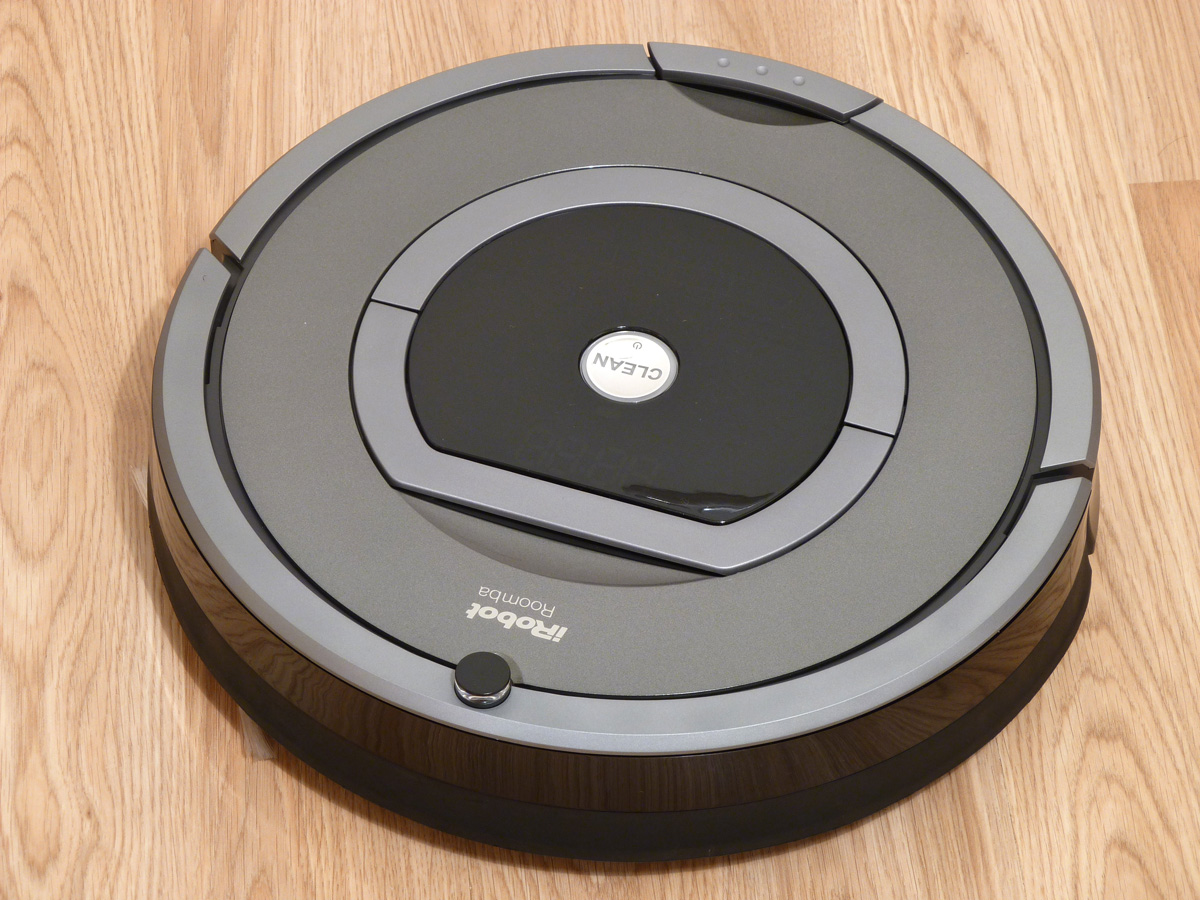
\includegraphics[width=0.6\textwidth]{img/roomba.jpg}
    \caption{Aspiradora robótica \textit{Roomba}} \label{fig:roomba}
    \end{figure}

    \item Robots médicos: Son robots diseñados para el uso en medicina para realizar tareas que requieren mucha precisión como en el caso de una cirugía, con el robot \textit{Da Vinci} o robots diminutos que son capaces de navegar por las venas hasta llegar al corazón y allí realizar la cirugía necesaria.
      \begin{figure}[H]
    \centering
    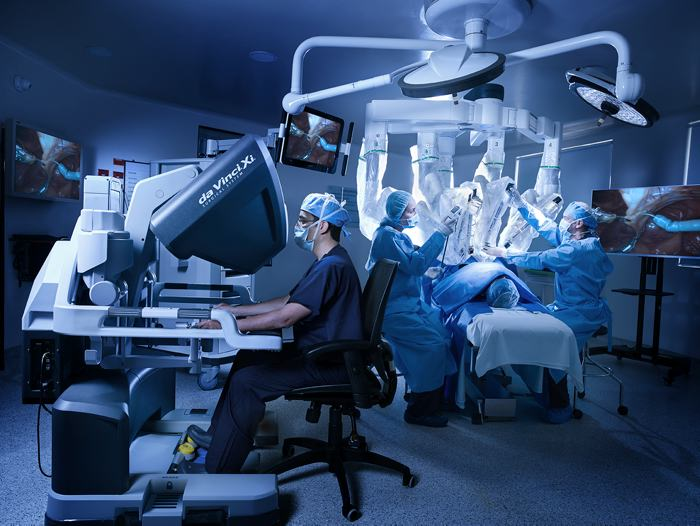
\includegraphics[width=0.6\textwidth]{img/davinci.jpg}
    \caption{Robot médico \textit{Da Vinci}} \label{fig:davinci}
    \end{figure}
    
    \item Robots militares: Son robots orientados a tareas militares, como reconocimientos de zonas conflictivas o rescate de personas, desactivación de bombas. En los últimos años también se han desarrollado mucho los drones en combate.
      \begin{figure}[H]
    \centering
    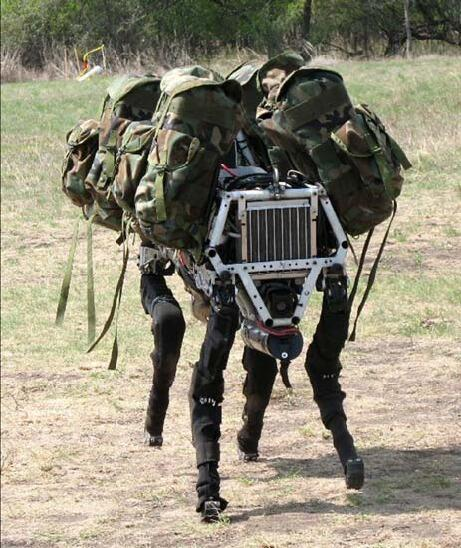
\includegraphics[width=0.6\textwidth]{img/bigdog.jpg}
    \caption{Robot militar \textit{Big Dog} creado por \textit{Boston Dynamics}} \label{fig:bigdog}
    \end{figure}
    
    \item Vehículos autónomos: Es el campo de la robótica que más en auge esta ahora mismo. El objetivo de estos robots es usar la información que proporcionan sus sensores como cámaras, sensores infrarrojos, sistemas \textit{Lidar} o el GPS entre otros, para llevar el vehículo de un lugar a otro.

    \begin{figure}[H]
        \centering
        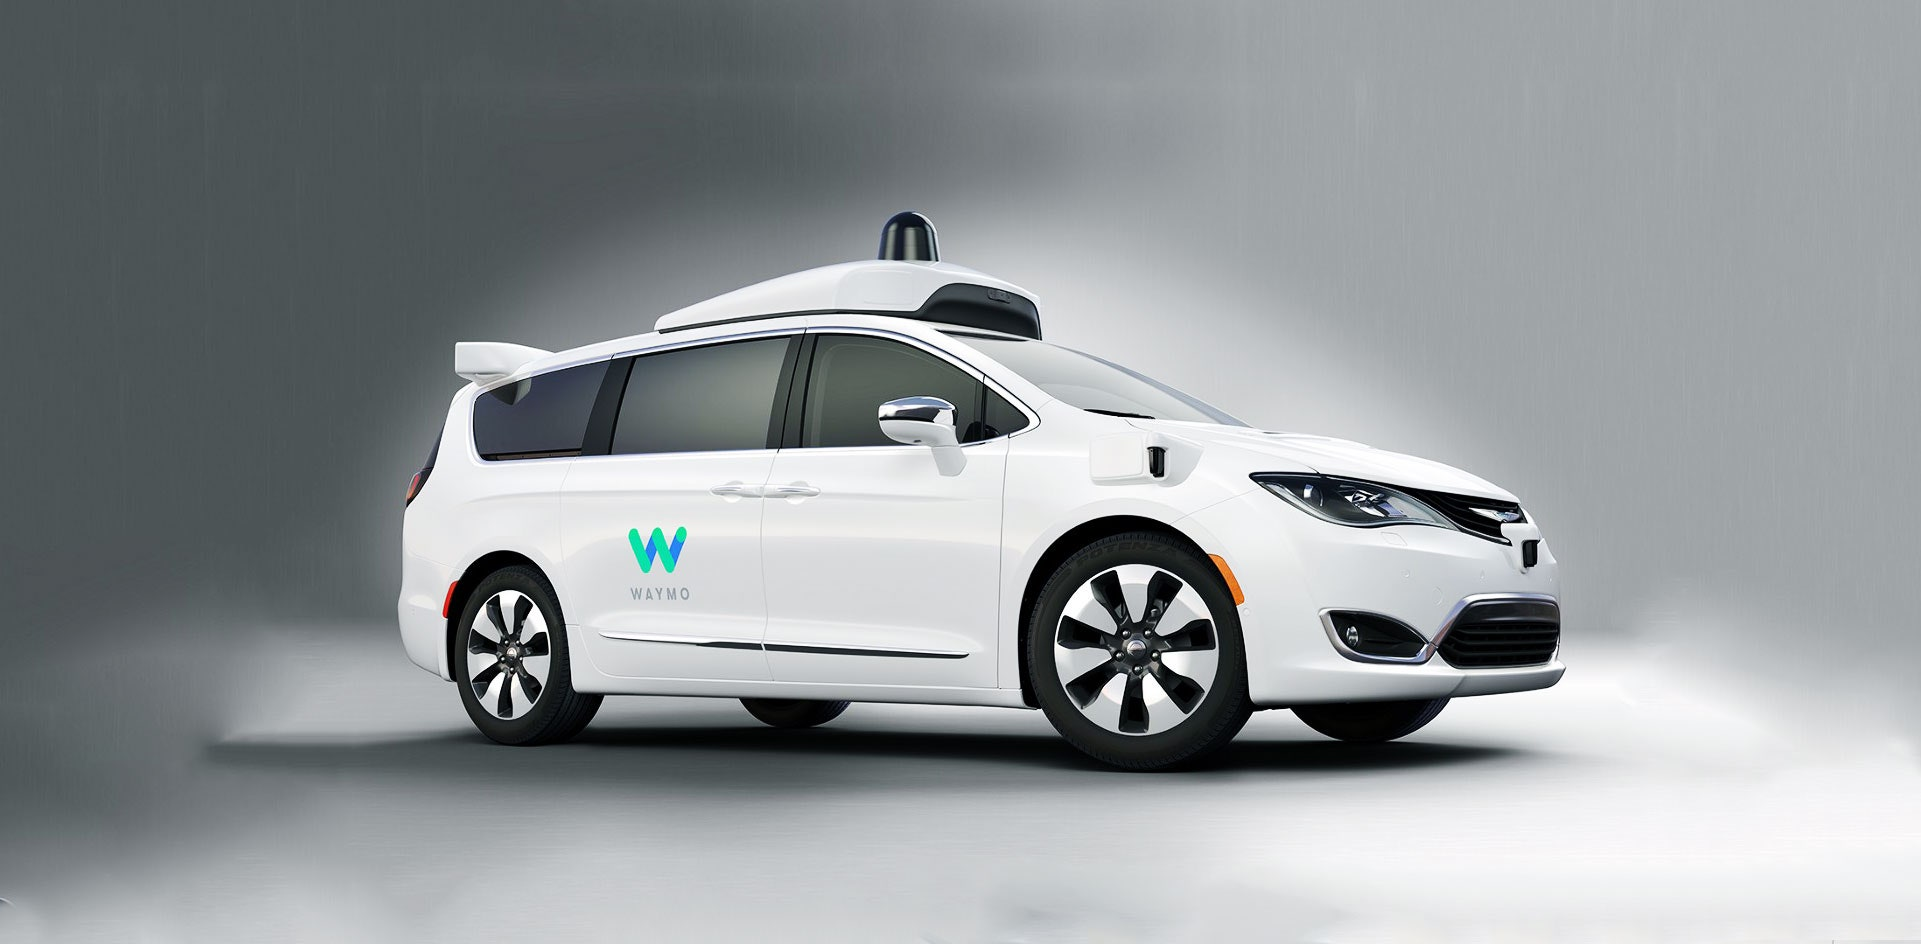
\includegraphics[width=0.7\textwidth]{img/waymo.jpg}
        \caption{Vehículo \textit{Waymo} de \textit{Google}} \label{fig:waymo}
    \end{figure}

    \item Robots Espaciales: Los famosos \textit{Rover} de la \textit{NASA} son robots diseñados para entornos donde el ser humano no puede llegar. Se centran en reconocimiento del terreno y análisis de las muestras que recogen.
        \begin{figure}[H]
    \centering
    \includegraphics[width=0.5\textwidth]{img/perseverance.jpg}
    \caption{Robot \textit{Perseverance} de la \textit{NASA}} \label{fig:Perseverance}
    \end{figure}
\end{itemize}

\subsection{Software en robótica}
\label{subsec:softwarerobot}
Para dotar de esta inteligencia a los robots se necesitan herramientas que transformen los datos recibidos de los sensores en algo que puedan aplicar en los actuadores. Hace años, cada máquina tenía un software específico con sensores y actuadores únicos para ese robot y esa tarea a desarrollar. Esto hacia, que aunque hubieras implementado el software para otros robots anteriormente, tuvieras que repetir el proceso con cada nuevo robot. Con los años se desarrollaron plataformas de software que permiten desarrollar de manera genérica para todos los robots, y actuando de mediador entre el robot y el software del creador,estos son los llamados \textit{middleware} que hacen que te puedas abstraer de los \textit{drivers} característicos de cada robot. Los middleware mas importantes a día de hoy son:
\begin{itemize}
    \item \textit{\textbf{Robot Operating System (ROS)}}\cite{bib:ros}. Plataforma de \textit{software} libre para el desarrollo de \textit{software} de robots. Provee servicios estándar de un sistema operativo como la abstracción de \textit{hardware}, control de dispositivos de bajo nivel, mecanismos de intercambio de mensajes entre procesos y mas herramientas vitales para el desarrollo del robot. Es el mas utilizado a día de hoy porque fue especialmente desarrollado para \textit{UNIX} y luego se implemento para el resto de sistemas operativos
    \item \textit{\textbf{ORCA}}\cite{bib:orca}. Plataforma de \textit{software} libre diseñado para crear aplicaciones mas complejas, ya que esta orientado a las componentes por separado
     \item \textit{\textbf{OROCOS}}\cite{bib:orocos} Proyecto de \textit{software} libre también orientado a componentes y basado en C++

\end{itemize}{}

\subsection{Simuladores robóticos}
\label{sec:simuladores}
La simulación  es el proceso de diseñar un modelo de un sistema real y llevar a término experiencias con él, con la finalidad de comprender el comportamiento del sistema o evaluar nuevas estrategias. De esta forma los simuladores ahorran tiempo porque puedes detectar posibles errores en el código antes de lanzarlo en el \textit{Hardware} y que pueda llevar a mayores problemas.\newline
Algunos de los simuladores que más se utilizan y más nos interesan en este proyecto:
\begin{itemize}
    \item \textbf{Gazebo}\cite{bib:gazebo}: Gazebo es un simulador de robótica 3D de código abierto. Gazebo fue un componente en el Proyecto Player desde 2004 hasta 2011. Gazebo integró el motor de física ODE, la representación de OpenGL y el código de soporte para la simulación de sensores y el control del actuador. También es importante destacar que tiene soporte para \texttt{ROS} lo que significa que puedes probar código real del robot en el simulador
    \begin{figure}[H]
    \centering
    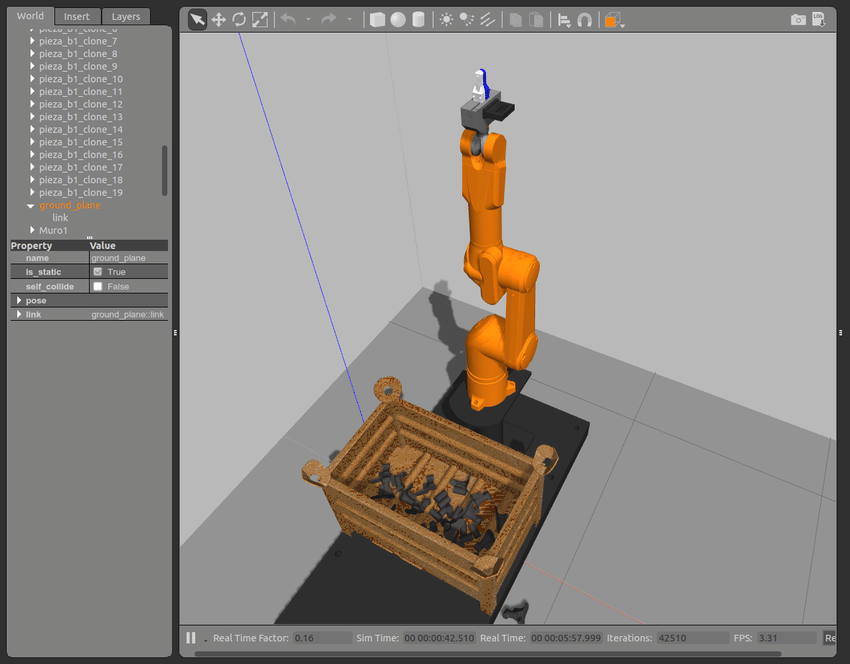
\includegraphics[width=0.7\textwidth]{img/gazebo.png}
    \caption{Interfaz de Gazebo} \label{fig:gazebo}
    \end{figure}
    
    \item \textbf{WebSim}: Es un simulador diseñado por alumnos de la universidad y que va escalando poco a poco. Hace uso de un entorno A-Frame y su diseño consiste en un editor que permite programar en diferentes lenguajes como \textit{JavaScript} y \textit{Python}, incluso un lenguaje de bloques llamado \textit{Blockly}(equivalente a Scratch pero diseñado por Google). Es la base de la plataforma de \textit{Kibotics} y que vamos a utilizar en este proyecto.
\end{itemize}

\section{Tecnologías web}
\label{sec:web}
Las tecnologías web sirven para acceder a los recursos de conocimiento que hay disponibles en \textit{Internet} utilizando un \textit{navegador}. Son herramientas que procesan y lo muestran mediante una interfaz gráfica lo almacenado en un servidor. Además gracias a la forma que esta estructurada la \textit{World Wide Web} (WWW) hace sencillo saltar de un recurso a otro. 
WWW es una combinación de 4 ideas: Hipertexto, identificadores de recursos(URL y URI), el lenguaje de marcado y el modelo cliente servidor.

\begin{figure}[h]
\centering
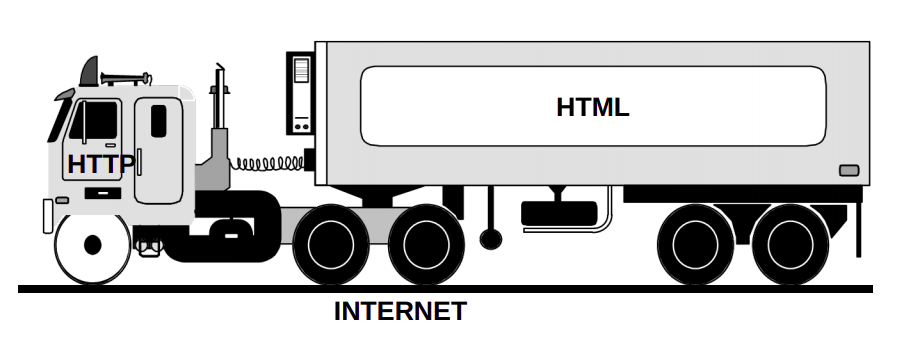
\includegraphics[scale=0.4]{img/tecnologiasweb.png}
\caption{Concepto de Tecnologias Web} \label{fig:tecnologiasweb}
\end{figure}

Lo que nos interesa de las \textit{Tecnologías Web} es el modelo de cliente-servidor, también llamado, \textit{FrontEnd} a todo lo que el usuario se encuentra directamente en la web, lo que es la parte del cliente. Y \textit{BackEnd} a la parte del interior de las aplicaciones que viven en el servidor, que es lo denominado \textit{el lado del servidor}. 
\subsection{FrontEnd}
\label{subsec:frontend} 
Es la parte encargada de dar forma a la interfaz de usuario y de establecer la comunicación con el servidor. Una pieza importante del cliente es el navegador, ya que es el encargado de leer e interpretar la información recibida. Entre los navegadores \textit{web} más empleados se encuentran \textit{Firefox}, \textit{Google Chrome} u \textit{Opera}\cite{bib:navegadores}. Las tecnologías que hacen posible esa comunicación son: 

\begin{itemize} 
    \item \textit{\textbf{JavaScript}}. Es un lenguaje de programación interpretado, dialecto del estándar ECMAScript. Se define como orientado a objetos. Es el lenguaje más utilizado para el desarrollo de aplicaciones Web y de paginas Web.
    \item \textit{\textbf{HTML}}. siglas en inglés de HyperText Markup Language, hace referencia al lenguaje de marcado para la elaboración de páginas web. Es el estándar más utilizado a día de hoy.\newline
HTML sólo sirve para indicar como va ordenado el contenido de una página web. Esto lo hace por medio de las marcas de hipertexto las cuales son etiquetas conocidas en inglés como tags. Las mejoras del diseño gráfico ya vienen dada de la versión actual, \textit{HTML5}, que incluye muchas mejoras respecto a su predecesor: \textit{canvas}, \textit{websockets}, \textit{WebRTC}, vídeo, audio, etc. Este lenguaje indica la estructura de una página web, para editar el estilo y presentación visual hay que hacer uso de otros elementos como \textit{CSS}.
    \item \textit{\textbf{Cascading Style Sheets (CSS)}}. Lenguaje de diseño gráfico para definir y crear la presentación de un documento escrito en un lenguaje de marcado. De esta forma, se puede separar información y datos (en los documentos \textit{HTML}) y todo lo relativo al diseño y presentación (en documentos \textit{CSS}). Actualmente los navegadores usan la versión \textit{CSS3}.

\end{itemize}

\begin{figure}[h]
\centering
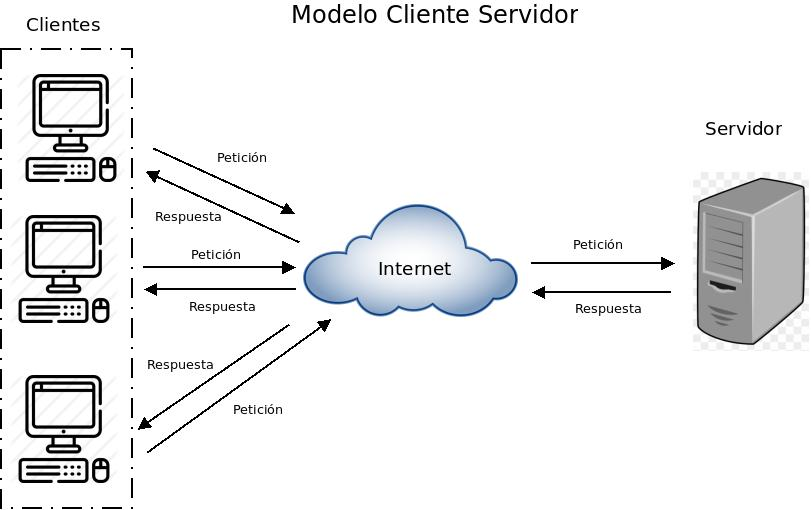
\includegraphics[scale=0.4]{img/http.jpeg}
\caption{Comunicación cliente-servidor en HTTP} \label{fig:http}
\end{figure}
\subsection{BackEnd}
\label{subsec:backend}
En la parte del servidor web se encarga de proveer los datos, hacer posible crear una aplicación que se le mostrará al cliente y facilitar herramientas como bases de datos y recursos compartidos. 
\begin{itemize}
    \item \textbf{Node.js}: Node. js es un entorno JavaScript que nos permite ejecutar en el servidor, de manera asíncrona, con una arquitectura orientada a eventos   
    \item \textbf{Django}: Django es un entorno web extremadamente popular y completamente funcional, escrito en  \textit{Python}. 
\end{itemize}

\subsection{HTTP}
\label{subsec:http}

\textit{HiperText Transfer Protocol} (\textit{HTTP}) es el protocolo de nivel de aplicación utilizado para transferir recursos hipermedia entre ordenadores y sigue el esquema petición-respuesta entre cliente y servidor (Figura \ref{fig:http}). 
Las peticiones están definidas por el protocolo y tienen métodos concretos: 
\begin{itemize}
    \item GET: Solicita un recurso al servidor especificando su \textit{URL}.
    \item HEAD: Método similar a GET con la diferencia de que únicamente solicita las cabeceras y no descarga el recurso completo.
    \item POST: Envía datos al servidor, normalmente un recurso específico que provoca un cambio de estado. Es también bastante similar GET pero la cabecera va en claro. 
    \item PUT: Actualiza información sobre un recurso del servidor. 
    \item DELETE: Elimina en el servidor un recurso.
\end{itemize}

Aunque estos son los principales métodos, el protocolo tiene flexibilidad para ir añadiendo nuevos e incorporar funcionalidad. El número de métodos ha ido aumentando con las nuevas versiones.\newline




\section{Robótica educativa}
\label{sec:educativa}
La robótica educativa ha ido tomando mas importancia con los años, ya que cada vez es más importante que estudiantes de cualquier nivel estén familiarizados con la tecnología, tiene valores positivos como la implementación de pensamiento lógico, resolución de problemas y trabajo en equipo en las actividades académicas, que son ramas del conocimiento que se desarrollan poco en edades tempranas , con una componente en conocimiento matemático y físicos y además añade un atractivo que no tienen las asignaturas convencionales.
Muchos estudios han demostrado que el uso de kits de robótica en la educación favorece a la capacidad de reflexión de los estudiantes.
Cada año se crean mas cursos de robótica, y en 2015 la comunidad de Madrid introdujo la asignatura de robótica en los planes docentes de Enseñanza Secundaria con la asignatura ``Tecnología, Programación y Robótica'' y en el curso 2020-2021 se empezará a implantar en Educación Primaria la asignatura ``Programación y Robótica''.\newline
Este tipo de educación es el llamado modelo \textbf{STEM} (siglas de \textit{Science, Technology, Engineering y Mathematics}), término creado por Seymound Papert en la década de los 80 cuando creo uno de los primeros juguetes con programación incorporada, creada para niños, el llamado \textit{"Lego-Logo"}, dando mucha importancia a juegos con engranajes, que consideraba que enriquecía el pensamiento. Justamente, el referente del protagonista de este proyecto.\newline
Pero no fue hasta 2010, cuando este modelo de educación empezó a tomar relevancia, y se inicio la inclusión en la agenda escolar.
        \begin{figure}[H]
    \centering
    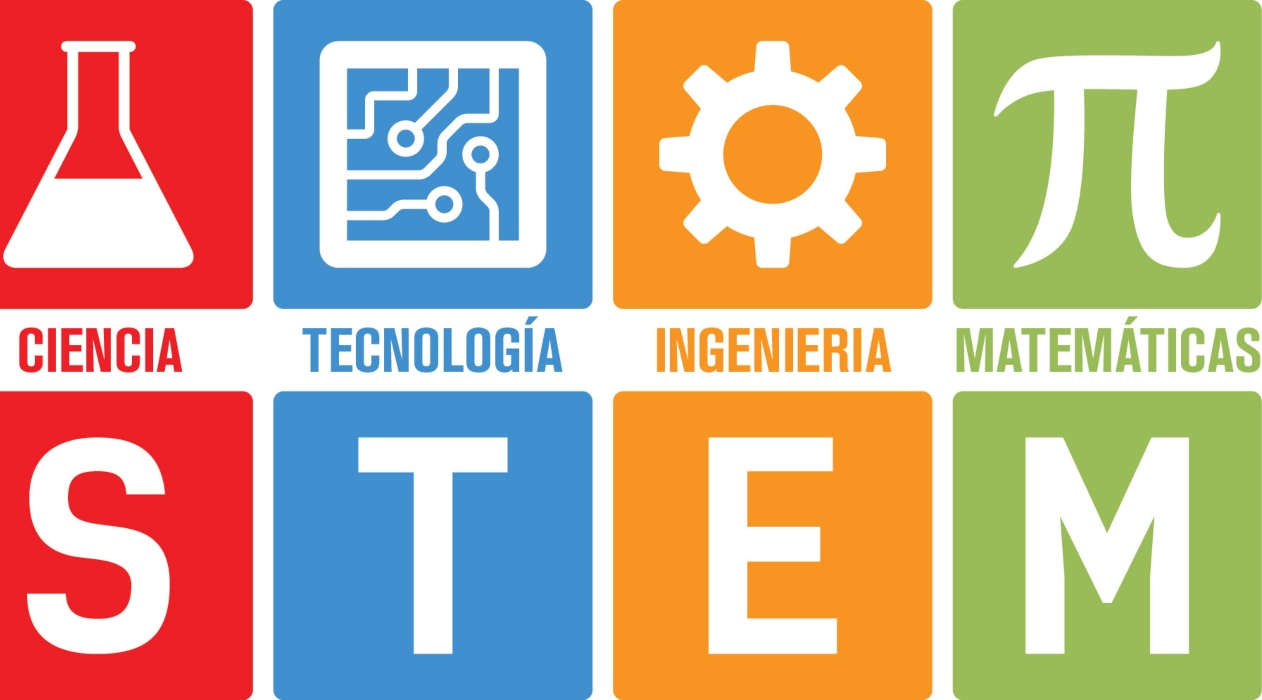
\includegraphics[width=0.7\textwidth]{img/stem.jpg}
    \caption{Modelo de Educación \textit{STEM}} \label{fig:stem}
    \end{figure}
Una de las mayores partes de la robótica tiene que ver con la programación, que además de ser una habilidad muy importante para la sociedad actual, es algo complejo. Por lo que se utilizan lenguajes de programación visual, estos se tratan de lenguajes que abstraen en bloques las funciones o métodos de cualquier lenguaje de programación. Dentro de este tipo de lenguajes, los más destacables son :

\begin{itemize}
    \item \textit{\textbf{Scratch}}\cite{bib:scratch}: proyecto liderado por el Grupo \textit{Lifelong Kindergarten} del \textit{MIT}, es utilizado por estudiantes para programar animaciones, juegos e interacciones. Su atractivo reside en lo fácil que es de entender el pensamiento computacional debido a su sencilla interfaz gráfica y la implementación de sus bloques.
    \begin{figure}[H]
    \centering
    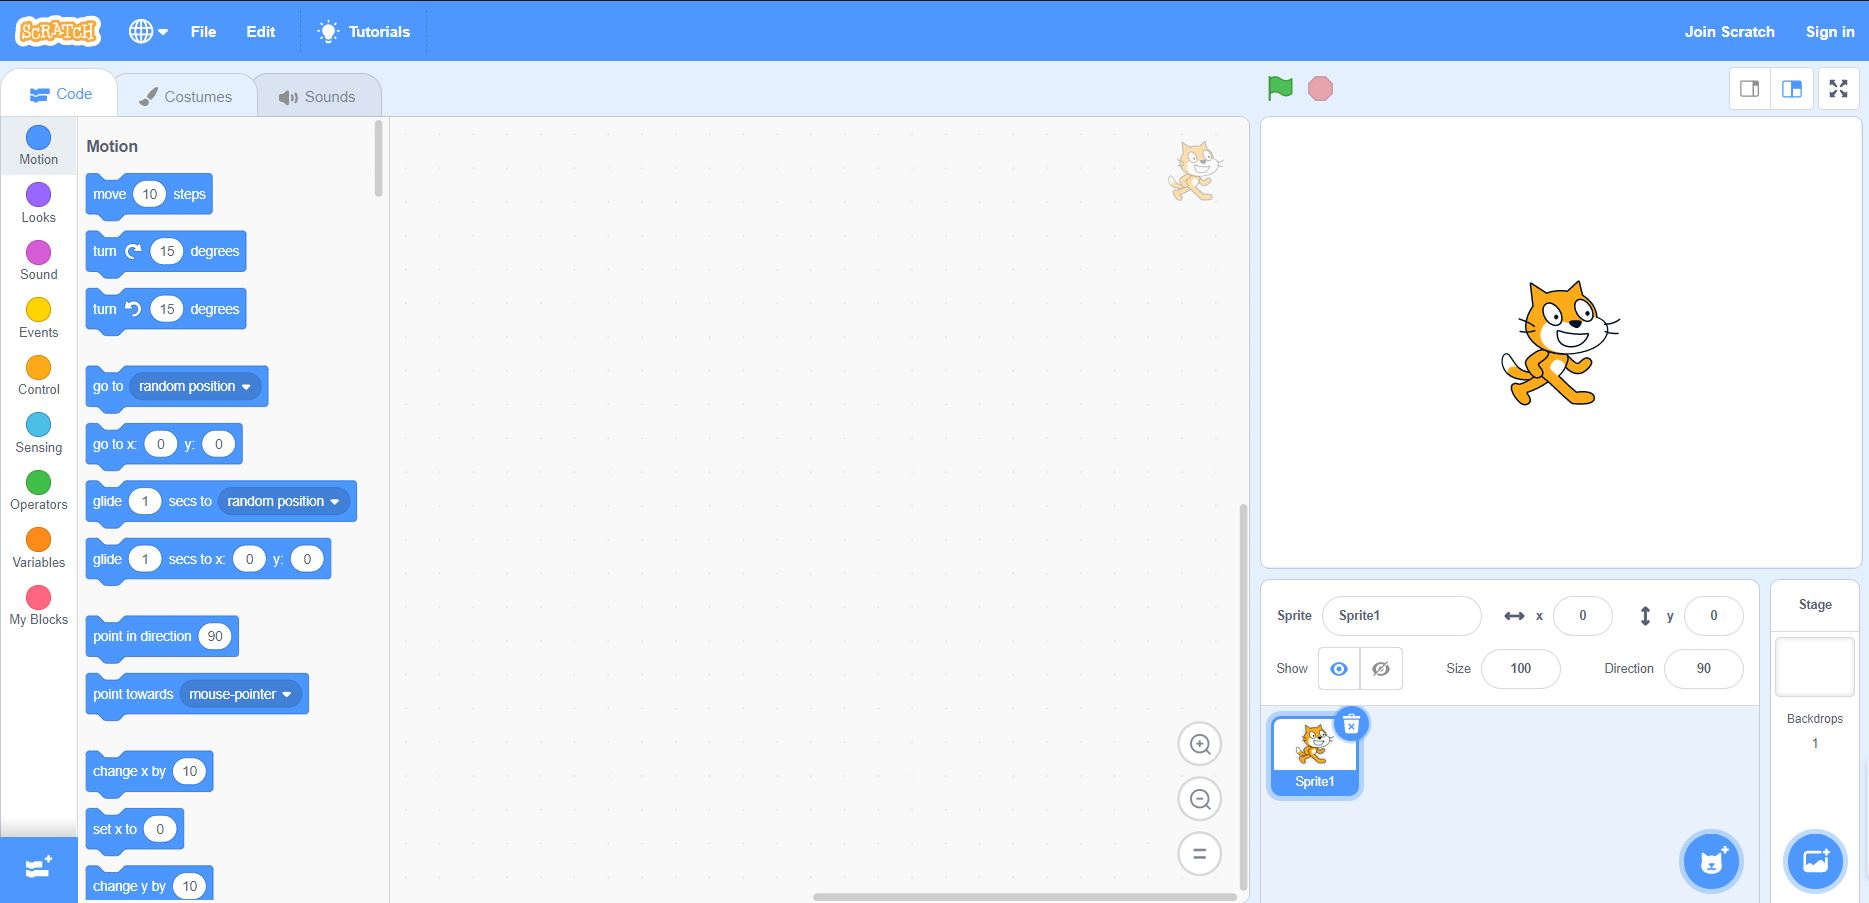
\includegraphics[width=0.7\textwidth]{img/scratch.jpg}
    \caption{Interfaz gráfica de Scratch} \label{fig:scratch}
    \end{figure}

    \item \textit{\textbf{LEGO}}\cite{bib:lego}: Es el robot base de este proyecto,dispone de una amplia gama de robots programables y cada uno de ellos tiene un sistema gráfico, que es similar entre ellos pero también ligado a la edad el estudiante para el que esta diseñado el software. 

    \begin{figure}[H]
    \centering
    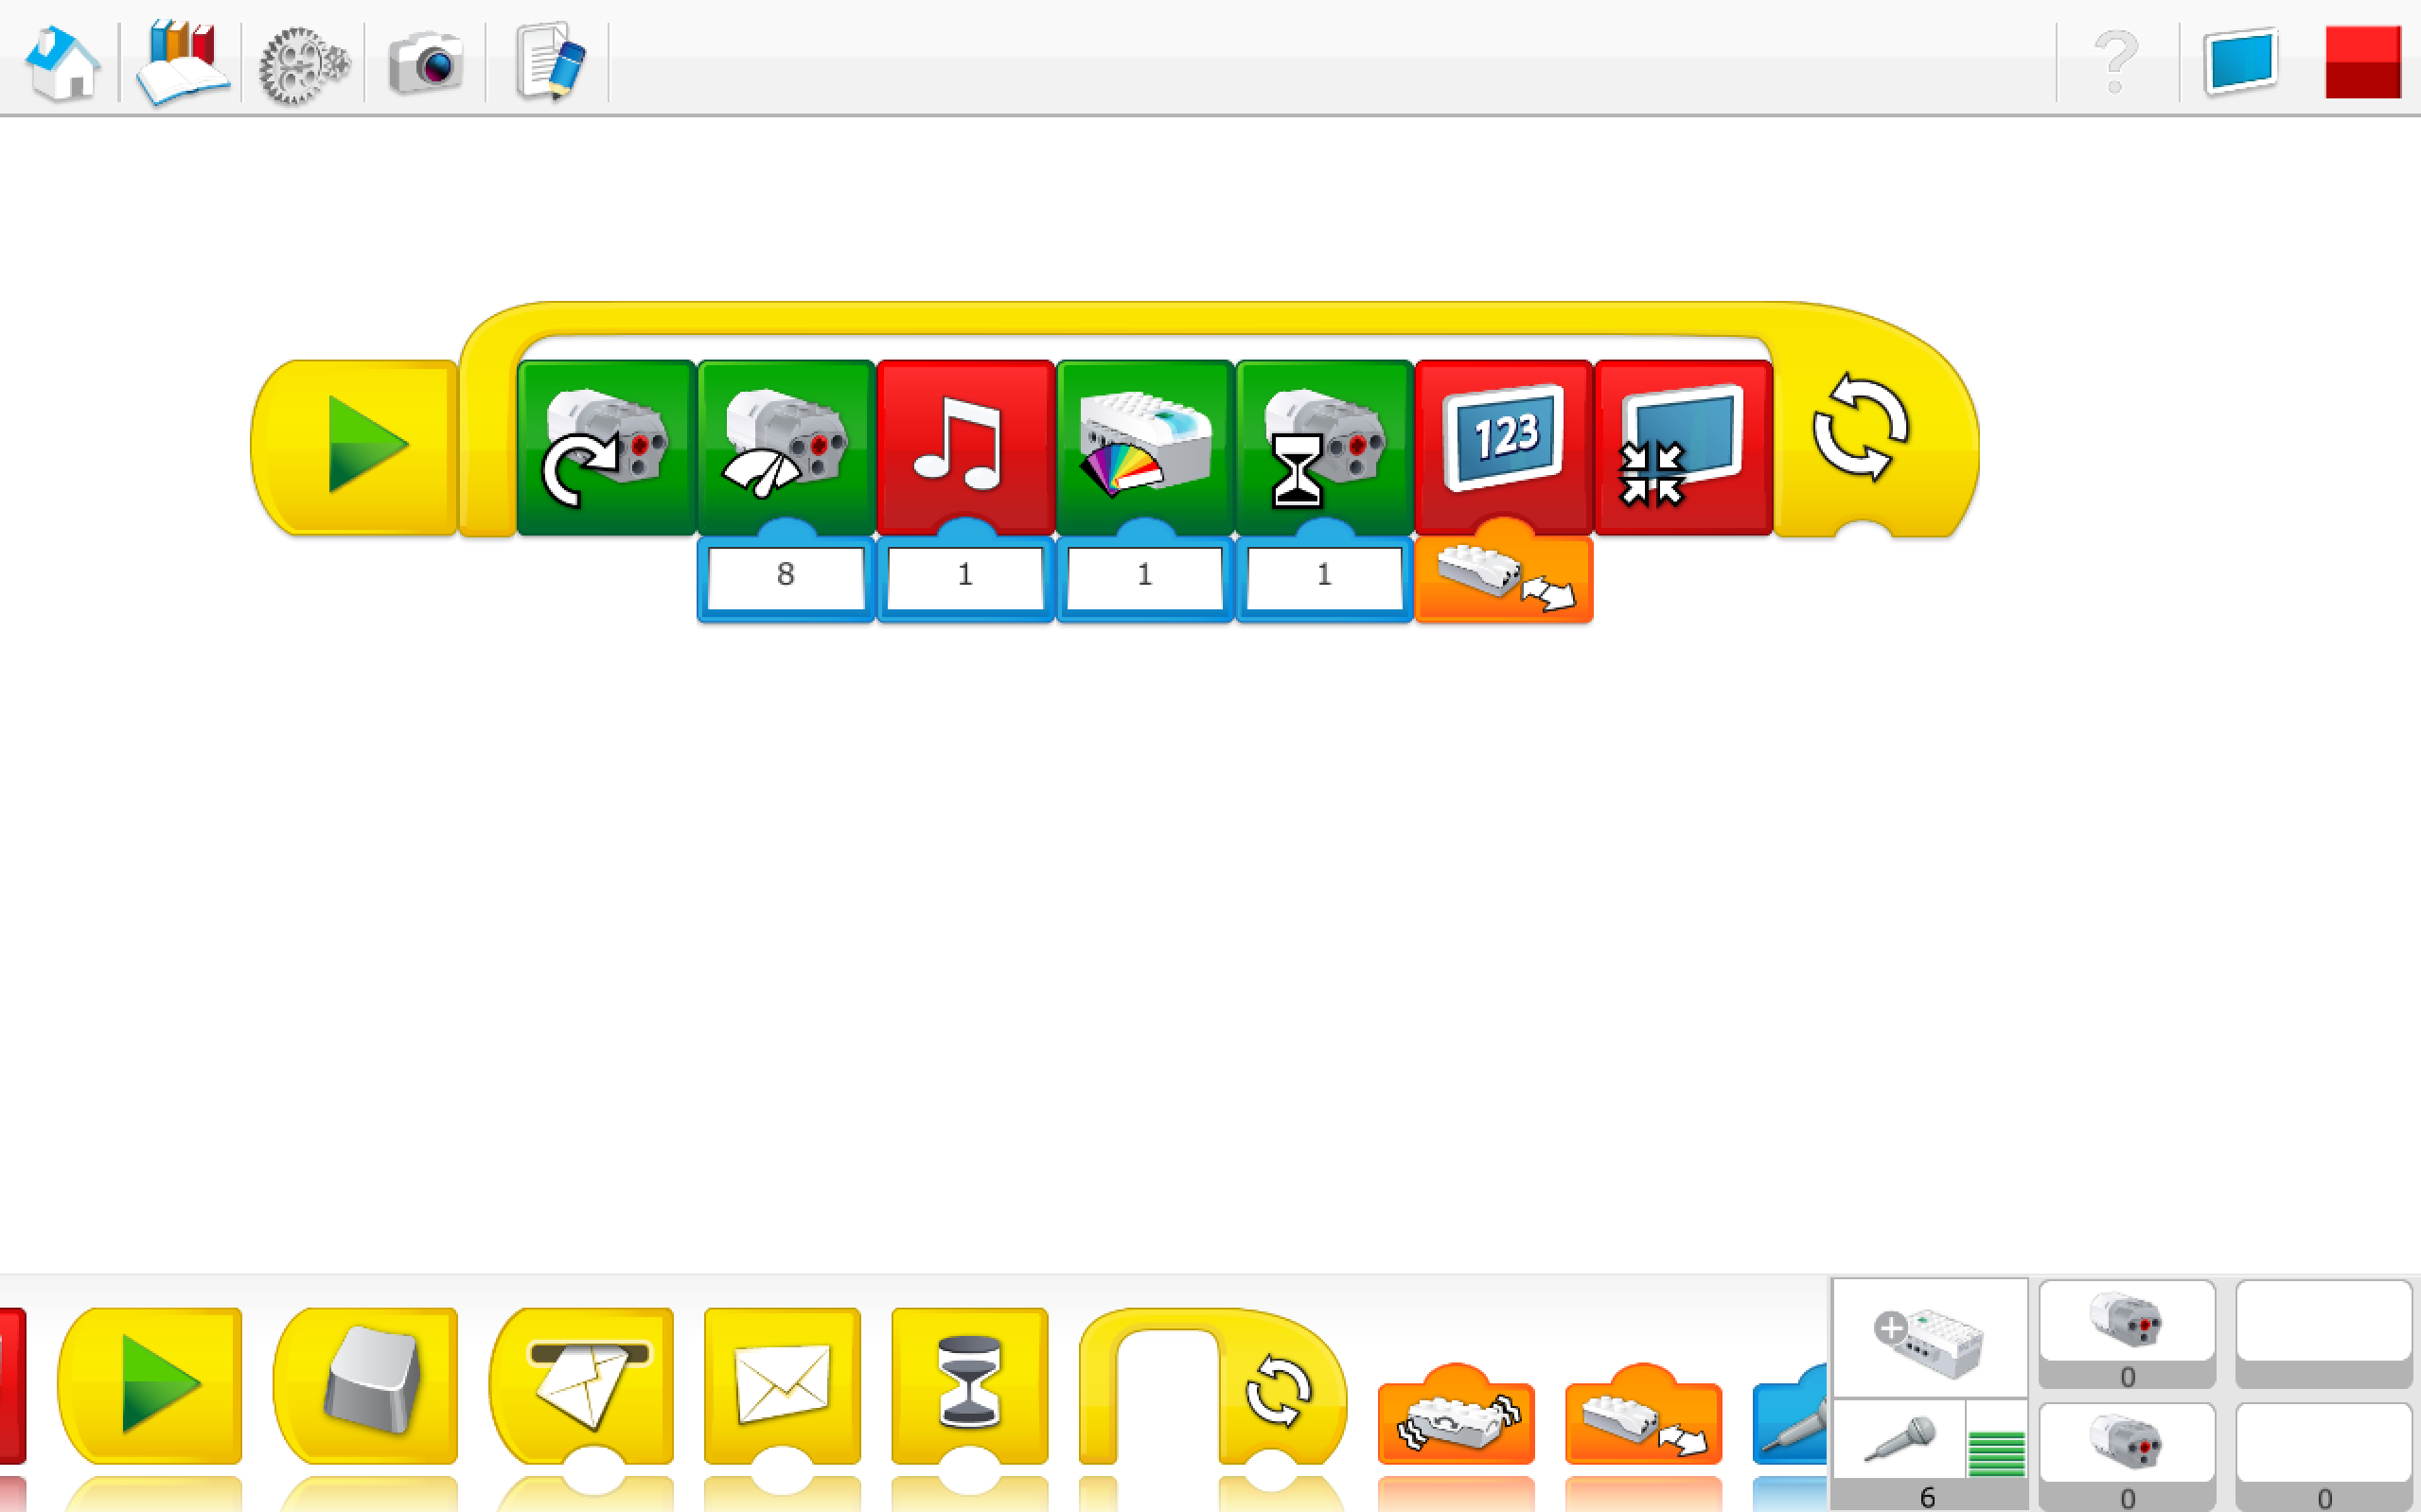
\includegraphics[width=0.7\textwidth]{img/lego1.png}
    \caption{Interfaz de LEGO WeDo} \label{fig:lego1}
    \end{figure}
    
Por ejemplo en la figura \ref{fig:lego1} se puede ver que la interfaz en este caso, es con colores vivos, los cuales representan distintas funcionalidades dentro del robot, es decir, el amarillo representa las acciones propias de programación, como: inicio de programa, fin de programa, bucles, esperar, etcétera. El color rojo representa los sensores del robot, todo lo que recoja datos. Y el color verde representa los motores que equivalen a los actuadores en este robot.
Como se puede observar es una abstracción muy simple para estudiantes de mas corta edad.
	 \begin{figure}[H]
    \centering
    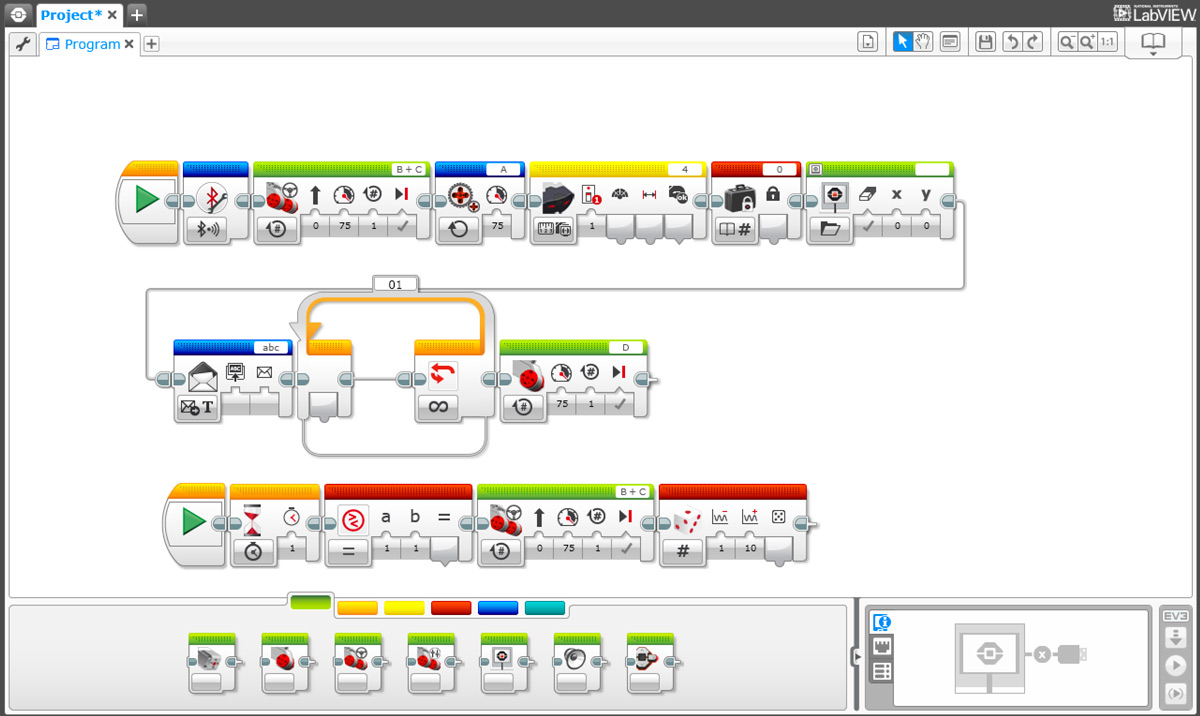
\includegraphics[width=0.7\textwidth]{img/lego2.jpg}
    \caption{Interfaz gráfica de LEGO Ev3} \label{fig:lego2}
    \end{figure}

En el caso del software para el \textbf{LEGO Ev3}, añade un grado de complejidad, incluyendo apartados para realizar operaciones matemáticas, envío de archivos entre robots, y más actuadores, como la pantalla que integra el robot, o los altavoces.

En el caso de LEGO y en otros kits incorporan los elementos básicos para la construcción de un robot. En este en particular viene con lo indispensable para construir con piezas de LEGO. También incluye un microprocesador para ser programado, con Linux instalado, sensores (infrarrojos, táctiles y de color) y motores.
  \begin{figure}[H]
    \centering
    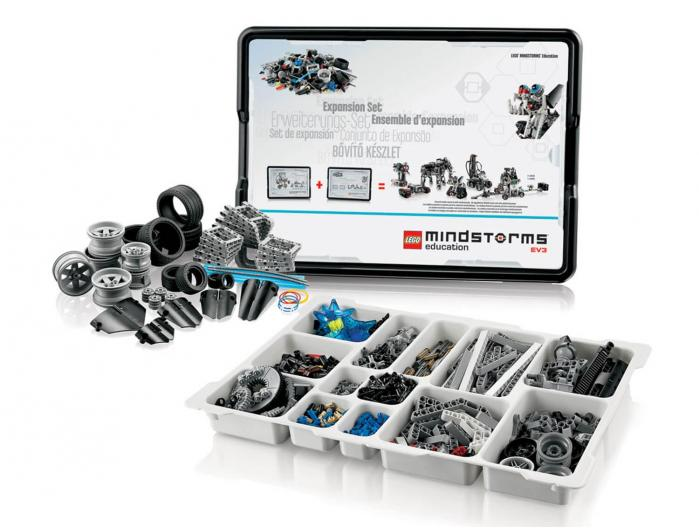
\includegraphics[width=0.7\textwidth]{img/kitev3.jpg}
    \caption{Kit de piezas y sensores de LEGO Ev3} \label{fig:lego3}
    \end{figure}
\end{itemize}{}


En el siguiente capitulo, profundizaré más en lo que se puede hacer con el robot \textbf{LEGO Ev3} y explicaré cuales van a ser los objetivos y porque elegir este robot.



\subsection{Kibotics}
\label{sec:kibotics}
Kibotics\footnote{\url{https://kibotics.org/}}\cite{bib:kibotics}, es un entorno web desarrollado por la Asociación JdeRobot\footnote{\url{https://jderobot.github.io/}} para la docencia de robótica. Fue creada para impartir cursos de robótica, en los que destacan una iniciación muy sencilla, y una gran variedad de recursos a disposición del alumno.
Es una plataforma en la que podemos encontrar distintos ejercicios de robots simulados que no son reales (como el Formula 1). Tiene los ejercicios divididos , en los robots con ruedas sobre una superficie, con cámaras, sensores de todo tipo, y los drones, con funcionalidad adicional, y otro tipo de ejercicios, y dentro de estos dos grupos, se dividen entre los dos lenguajes de programación. \newline
 
\begin{figure}[h]
  \centering
    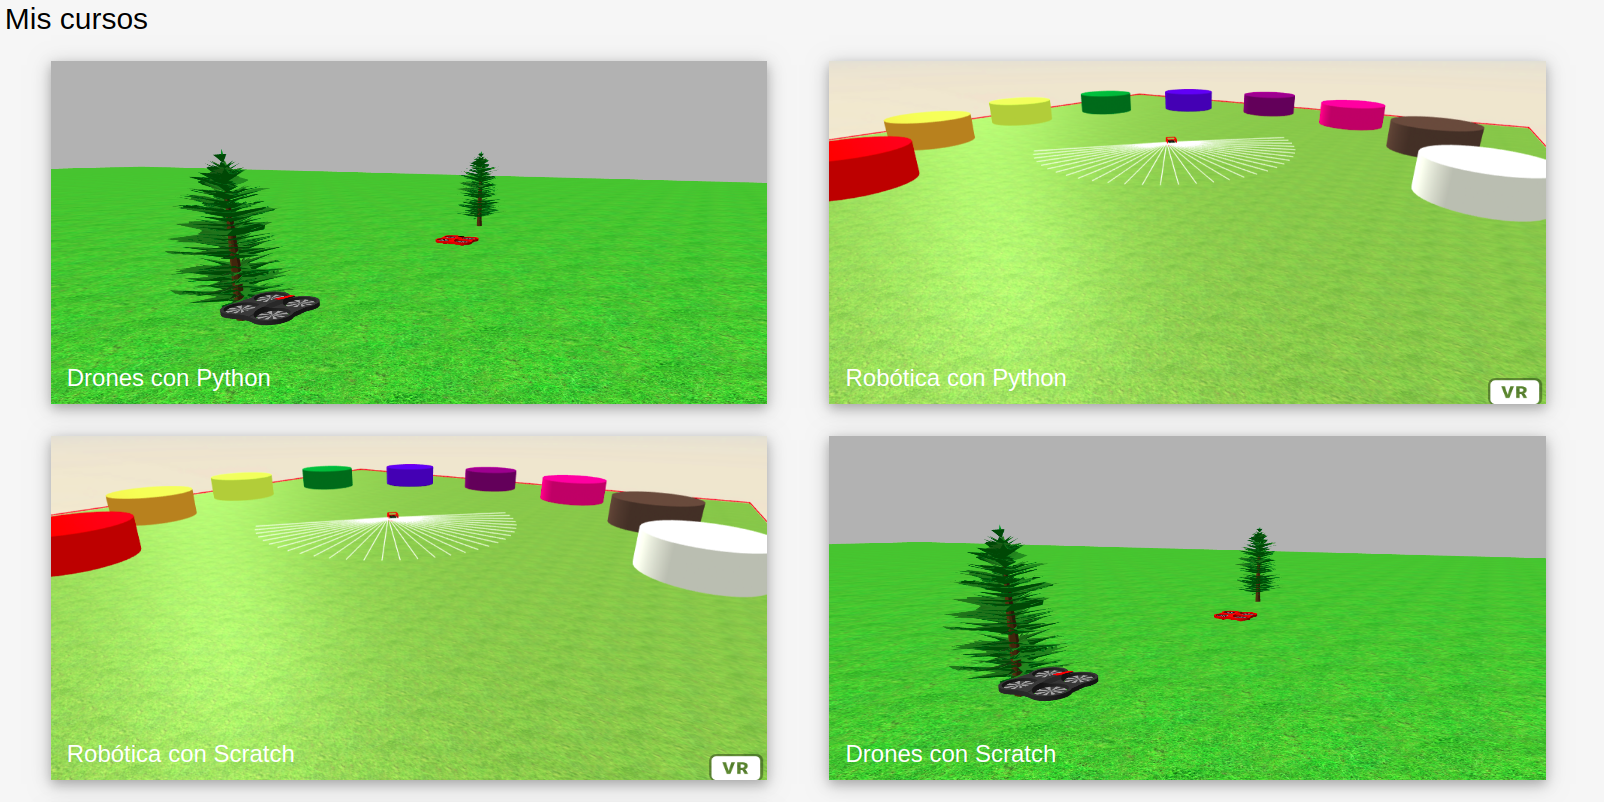
\includegraphics[width=1\textwidth]{img/kibotics2.png}
  \caption{Menu principal de \textit{Kibotics}}
  \label{Robot PiBot}
\end{figure}
En cuanto a los lenguajes reconocidos por esta plataforma, encontramos \textit{Blockly},el equivalente de \textit{Scratch} pero creada por \textit{Google}, un lenguaje de bloques. Su uso en colegios, para estudiantes de corta edad es cada vez más frecuente. También encontramos \textit{Python} un lenguaje de alto nivel, de los más populares actualmente. Es el que emplean los estudiantes más mayores. 
\begin{figure}[h]
  \centering
    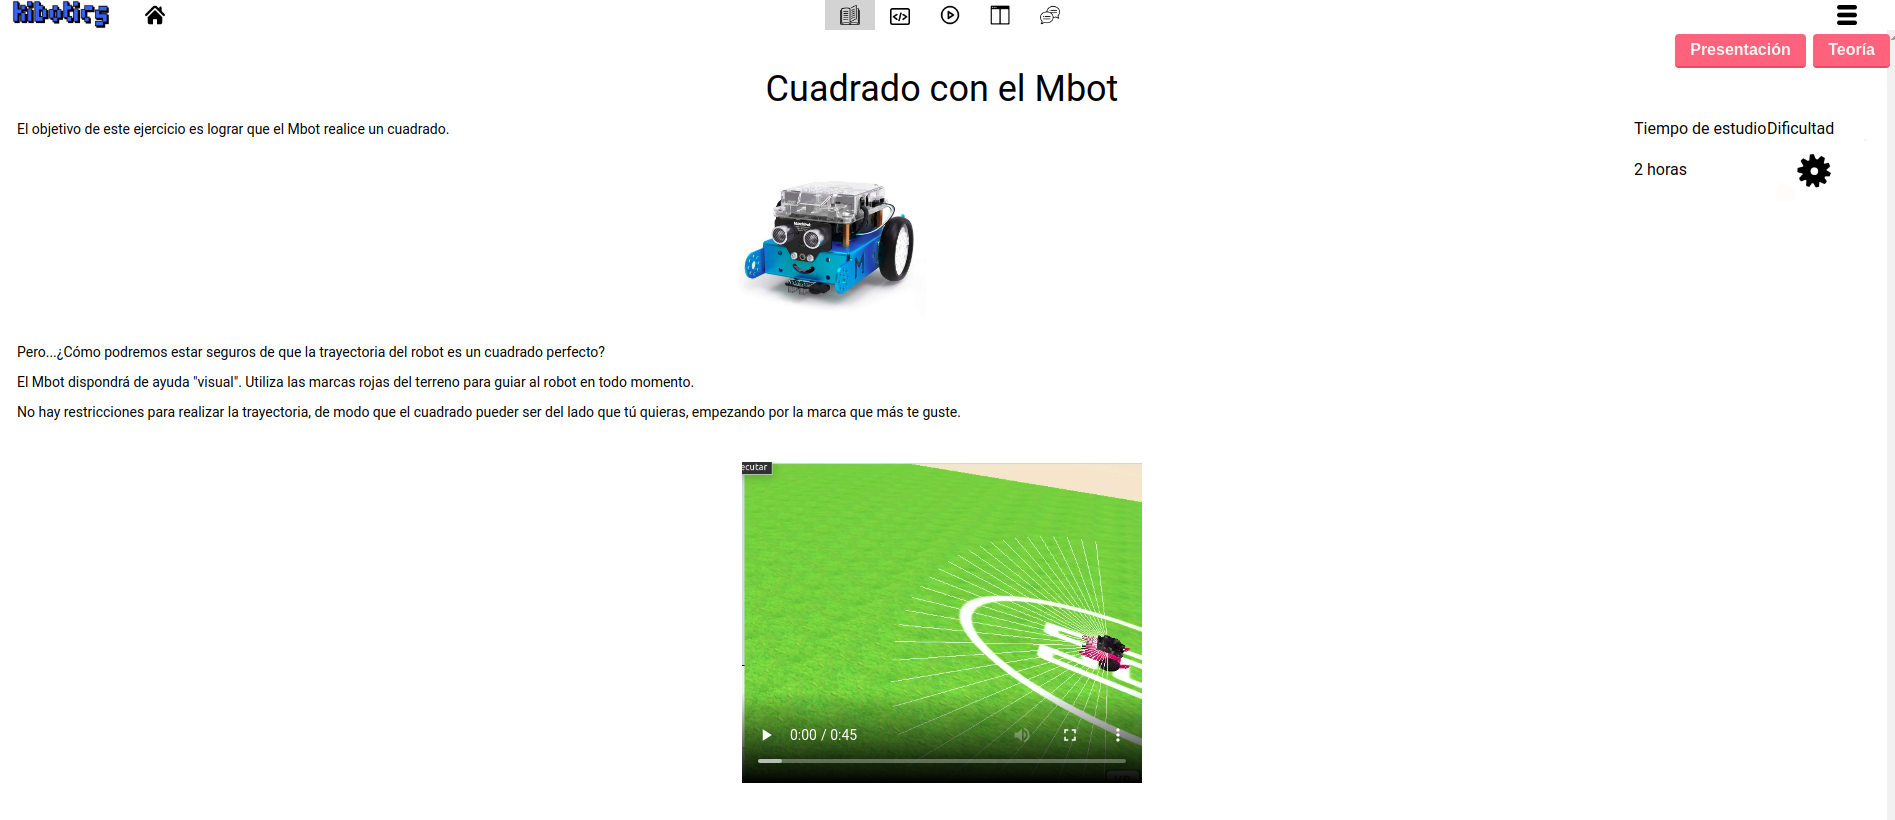
\includegraphics[width=1\textwidth]{img/kibotics1.png}
  \caption{Ejercicio en Kibotics}
  \label{Ejercicio con Blockly en Kibotics}
\end{figure}

Cada ejercicio viene con una parte teórica, donde se explica la lección que se va a aprender y los pasos para seguir para poder completar el ejercicio, la siguiente pestaña, es donde se programa el ejercicio, y la última, es donde se encuentra el simulador que ejecuta el código que acabas de programar.




